\documentclass[11pt]{article}


\usepackage{latexsym}
\usepackage[margin=1in]{geometry}
\usepackage{graphicx}
\usepackage{subfig}
\usepackage{enumerate}
\usepackage{mathptmx}
\usepackage{amsmath}
\usepackage{amsfonts}
\usepackage{amssymb}
\usepackage{amsbsy}
\usepackage{amsthm}
\usepackage[pdftex,colorlinks=true,urlcolor=blue,citecolor=black,anchorcolor=black,linkcolor=black]{hyperref}


\newtheorem{theorem}{Theorem}
\renewcommand{\thetheorem}{ \arabic{theorem}}
\newtheorem{corollary}[theorem]{Corollary}
\renewcommand{\thecorollary}{\arabic{corollary}}
\newtheorem{definition}{Definition}
\renewcommand{\thedefinition}{\arabic{definition}}
\newtheorem{lemma}{Lemma}
\renewcommand{\thelemma}{ \arabic{lemma}}
\newtheorem{proposition}{Proposition}
\renewcommand{\theproposition}{ \arabic{proposition}}
\newtheorem{remark}{Remark}
\renewcommand{\theremark}{ \arabic{remark}}

% Frequently used general mathematics
\newcommand{\R}{{\mathbb{R}}}
\newcommand{\Rp}{\R^+}
\newcommand{\Z}{{\mathbb{Z}}}
\newcommand{\Zp}{\Z^+}
\newcommand{\Q}{\mathbb{Q}}
\newcommand{\N}{\mathbb{N}}

% Commands for probability
\newcommand{\p}[1]{\mathbb{P} \left\{ #1 \right\}}
\newcommand{\e}[1]{\mathbb{E} %\left[ 
#1 %\right]
}
\newcommand{\ee}[2]{\mathbb{E}_{#1} \left[ #2 \right]}
\newcommand{\var}[1]{\mathrm{Var} \left( #1 \right)}
\newcommand{\cov}[1]{\mathrm{Cov} \left( #1 \right)}
\newcommand{\cor}[1]{\mathrm{Corr} \left( #1 \right)}
\newcommand{\varh}[1]{\widehat{\mathrm{Var}} \left( #1 \right)}
\newcommand{\vart}[1]{\widetilde{\mathrm{Var}} \left( #1 \right)}
\newcommand{\vartg}[1]{\widetilde{\mathrm{Var}}_\gamma \left( #1 \right)}
\newcommand{\varhat}{\widehat{\mathrm{Var}}}

% Definitions of variables
\newcommand{\X}{X}
\newcommand{\x}{x} %% CHANGED THIS NOT TO BE MATHBF 
\newcommand{\xh}{{\hat{\x}}}
\newcommand{\xs}{\x^*}
\newcommand{\xit}{\xi}  %% CHANGED THIS TO BE WITHOUT TILDE! 
\newcommand{\xiti}{\xit^i}
\newcommand{\zs}{z^*}
\newcommand{\nb}{\left\lfloor\tfrac{n-m}{\gamma}\right\rfloor+1}
\newcommand{\nbl}{\left\lfloor\tfrac{n_l-m_l}{\gamma_l}\right\rfloor+1}
\newcommand{\gammab}{\bar{\gamma}}
\newcommand{\ogb}{\tfrac{1}{\gammab}}
\newcommand{\cogb}{\left\lceil\ogb\right\rceil}

% Definitions for overlapping batches
\newcommand{\gb}{\bar{G}}
\newcommand{\gbb}{\bar{\gb}}
\newcommand{\db}{\bar{D}}
\newcommand{\dbb}{\bar{\db}}

% Used only for review of Meketon.  Should probably rewrite these.
%\newcommand{\xb}{\bar{x}}
%\newcommand{\xbb}{\bar{\xb}}
%\newcommand{\sx}{\{X_t, t \geq 0\}}
%\newcommand{\sxr}{\{X^n\}}
\newcommand{\y}{\mathbf{y}}
\newcommand{\yb}{\bar{y}}
\newcommand{\ybb}{\bar{\yb}}

\DeclareMathOperator*{\argmin}{argmin}

\newcommand{\Keywords}[1]{\par\noindent 
{\small{\em Keywords\/}: #1}}


%#########################################################
%*
%*  The Document.
%*
\begin{document}

\title{Overlapping Batches for the Assessment of Solution Quality in Stochastic Programs}

% AUTHOR: Enter the authors of the article, see end of the example document for further examples
\author{David~Love$^{a}$\ \ and G\"{u}zin~Bayraksan$^{b}$\thanks{Corresponding author. Tel.: +1 520-621-2605. Fax:+1 614-292-7852}\\[6pt]
{\small
      $^{a}$ Program in Applied Mathematics, University of Arizona, Tucson, AZ 85721, USA, \texttt{dlove@math.arizona.edu}} \\
{\small 
      $^{b}$ Integrated Systems Engineering, The Ohio State University, Columbus, OH 43210, USA, \texttt{bayraksan.1@osu.edu}}}

%% ONE WAY: JUST NAMES ON TOP, EVERYTHING ELSE AS FOOTNOTE
%\author{David~Love%
%\thanks{D.\ Love: Interdisciplinary Graduate Program in Applied Mathematics,
%University of Arizona, Tucson, AZ 85721, USA. E-mail: \texttt{dlove@math.arizona.edu}}%
%\ \ and G\"{u}zin~Bayraksan%
%\thanks{G.\ Bayraksan: (corresponding author) Department of Systems and Industrial Engineering, University of Arizona, Tucson, AZ 85721, USA. E-mail: \texttt{guzinb@sie.arizona.edu}. Tel.: +1 520-621-2605. Fax:+1 520-621-6555}}


%%  ANOTHER WAY: ALL ON TOP, TWO DIFFERENT ONES SIDE BY SIDE
%\author{David Love \\ [6pt]
%       \texttt{dlove@math.arizona.edu} \\
%        Program in Applied Mathematics \\
%        University of Arizona \\
%        Tucson, AZ 85721, USA \\
% Multiple authors are entered as follows.
% You may also need to adjust the titlevbox size in the preamble - search for titlevboxsize
%\and
%        G\"{u}zin Bayraksan \\ [6pt]
%        \texttt{guzinb@sie.arizona.edu} \\
%        Department of Systems and Industrial Engineering \\
%        University of Arizona \\
%        Tucson, AZ 85721, USA
%}
\date{}

\maketitle

\begin{abstract}
We investigate the use of overlapping batches for assessing solution quality in stochastic programs. 
Motivated by the original use of overlapping batches in simulation, we present a variant of the multiple replications procedure that reuses data via variably overlapping batches to obtain alternative variance estimators.  
These estimators have asymptotically lower variances, where the degree of variance reduction depends on the amount of overlap.  
We provide several desired asymptotic properties and present computational results to examine small-sample behavior.\smallskip 
	
	\Keywords{Sample average approximation; Optimality gap estimation; Overlapping batches; Stochastic programming}
\end{abstract}

%%%%%%%%%%%%%%%%%%%%%%%%%%%%%%%%%%%%%%%%%%%%%%%%%%%%%%%%%%%%%%%%%%%%%%%%%%%%%%%%
\section{Introduction}
\label{sec:intro}

We consider a stochastic program of the form
\begin{align} \tag{SP} \label{eq:sto_prog} 
	z^* & = \min_{\x \in X} \e{f(\x,\xit)},
\end{align}
where $\x$ is a vector of decision variables, $\xit$ is a vector of random variables, and $X$ is the feasible set, which is assumed to be independent of $\xit$.  
Further, it is assumed that the distribution of $\xit$ is known and that we can sample from it.  
Even though we will impose a more restrictive moment condition later, we assume that $\e{f(\x,\xit)}$ is well defined and finite for all $\x \in X$ and (\ref{eq:sto_prog}) has a finite optimal solution achieved on $X$.  
Let $\xit^1, \xit^2, \dots, \xit^m$ be an independent and identically distributed (iid) sample from the distribution of $\xit$.  
A sampling approximation of (\ref{eq:sto_prog}) is given by
\begin{align} \tag{SP$_m$} \label{eq:sto_prog_m}
	z_m^* & = \min_{\x \in X} \frac{1}{m} \sum_{i=1}^m f(\x,\xiti).
\end{align}
We denote an optimal solution to (\ref{eq:sto_prog}) as $\xs$ and an optimal solution to (\ref{eq:sto_prog_m}) as $\xs_m$.

We are interested in assessing the quality of a candidate solution $\xh \in X$, which may have been found in any way, defined by its optimality gap $\e{f(\xh,\xit)} - \zs$.  
This is important in practice since (\ref{eq:sto_prog}) typically cannot be solved exactly, so one only has an approximate solution $\xh$ without verification of its quality.  
Assessing solution quality is also a critical component of stopping criteria in algorithms.  
In many fields of optimization, it is common to evaluate an upper bound on the optimality gap through relaxations such as integrality or Lagrangian relations.  
In stochastic programming, given a sample size $m$, an upper bound on the optimality gap can be obtained by $\e{f(\xh,\xit)} - \zs \leq \e{f(\xh,\xit)} - \e{\zs_m}$ due to the inequality $\e{\zs_m} \leq \zs$.  
This bound improves as the sample size increases, that is, $\e{\zs_m} \leq \e{\zs_{m+1}} \leq \zs$ \cite{Mak1999,norkin_pflug_ruszczynski_98}.  
For stochastic programs, one way to estimate an upper bound on optimality gaps is through Monte Carlo sampling. 
A straightforward estimate of $\e{f(\xh,\xit)}$ is the sample mean, $\frac{1}{m} \sum_{i=1}^m f(\xh,\xiti)$. 
Instead of $\e{\zs_m}$, simply $\zs_m$ can be used.  
The resulting point estimator is  $G_m(\xh) = \frac{1}{m} \sum_{i=1}^m f(\xh,\xiti) - \zs_m$.  
Here, we assume the same observations $\xit^1, \dots, \xit^m$ are used in both terms of $G_m(\xh)$.  

Computing $G_m(\xh)$ involves solving an optimization problem (\ref{eq:sto_prog_m}) to obtain a lower bound estimator $\zs_m$, which complicates the statistical analysis. 
To enable statistical inference, the \emph{Multiple Replications Procedure} (MRP) of Mak et.\ al.\ \cite{Mak1999} generates $k$ independent estimators of $G_m(\xh)$, each using sample size $m$ and averages them to obtain a point estimator.  
To form confidence intervals, the sample variance of these estimators is calculated.  
This is essentially a nonoverlapping batch means type estimator ($k$ batches of size $m$) commonly used in simulation \cite{law_07}. 
We further review MRP estimators in \S \ref{ssec:mrp}.

In this paper, we extend MRP by overlapping the batches similar to the overlapping batch means (OBM) introduced by Meketon and Schmeiser \cite{Meketon1984}. 
Suppose each batch contains $m$ observations and that there are a total of $2m$ observations.  
In the nonoverlapping case, there are only two batches: the first batch contains observations $\xit^1, \xit^2, \dots, \xit^m$ and the second batch contains observations $\xit^{m+1}, \xit^{m+2}, \dots, \xit^{2m}$.   
Meketon and Schmeiser \cite{Meketon1984} overlap the batches so that the first batch is as before, the second batch now consists of $\xit^2, \xit^3, \dots, \xit^{m+1}$, the third batch contains observations $\xit^3, \xit^4, \dots, \xit^{m+2}$ and so on. 
As a result, the corresponding batch means are no longer independent. 
However, by simply reusing the data in this fashion, and seemingly in a contradictory way that induces dependence, one obtains a better variance estimator: a variance estimator that asymptotically has two-thirds of the variance of the usual batch means variance estimator but the bias of the two estimators is approximately the same.  
The idea of overlapping batches can be used for variance estimators of non-means \cite{SAH90} and recently, has been extended to estimators based on standardized time series (e.g., area, Cram\'{e}r-von Mises) for steady-state simulation output analysis \cite{Alexopoulos01012007,Alexopoulos2007}. 
In this paper, we explore its use for assessing solution quality in stochastic programs.  
Similar to Welch \cite{Welch1987} and Song and Schmeiser \cite{Song1992}, we consider partial overlap between batches to reduce computational effort in our setting. 
We present conditions under which the point estimators are strongly consistent (that is, they converge almost surely (a.s.) as opposed in to in probability; referred to simply as consistent from this point on), the same variance reduction benefits are achieved, and the resulting confidence intervals are asymptotically valid.  
We present computational results on two-stage stochastic linear and integer programs with recourse to examine small sample behavior.  
Our experiments indicate that the asymptotic variance reduction is achieved with small sample sizes, while bias and coverage probability are unaffected.

The rest of the paper is organized as follows.  
In the next section, we review relevant background information.  
We first discuss the overlapping batch means in \S \ref{ssec:obm} and then briefly go over the multiple replications procedure in \S \ref{ssec:mrp}.  
In \S \ref{sec:omrp}, we present the overlapping multiple replications procedure (OMRP) with variable overlap.  
In \S \ref{sec:theory}, we prove several asymptotic properties of the OMRP estimators and in \S \ref{sec:comp}, we test the performance of OMRP on three problems.  
We end in \S \ref{sec:concl} with a summary and conclusions.

%%%%%%%%%%%%%%%%%%%%%%%%%%%%%%%%%%%%%%%%%%%%%%%%%%%%%%%%%%%%%%%%%%%%%%%%%%%%%%%%
\section{Background}
\label{sec:background}

\subsection{Overlapping Batch Means} \label{ssec:obm}
Consider a covariance stationary stochastic process which has mean $\mu$ and variance $\sigma^2$.  
The task is to estimate $\mu$ given some realization of the stochastic process $\y = (y^1, y^2, \dots, y^n)$.  
Typically, this involves forming a confidence interval of the form $[L_\alpha(\y), U_\alpha(\y)]$ for a given level of significance $\alpha$ such that $\p{L_\alpha(\y) \leq \mu \leq U_\alpha(\y)} = 1 - \alpha$.  
The usual estimator for $\mu$ is the sample mean $\ybb = \frac{1}{n} \sum_{i=1}^n y^i$, which is an unbiased estimator even in the presence of correlated data.  
However, the usual variance estimator $\frac{1}{n-1} \sum_{i=1}^n (y^i - \ybb)^2$ can be inappropriate to use in the presence of correlated data, resulting in inaccurate interval estimators.  
To overcome this difficulty, various variance estimators have been proposed in the simulation literature; see, e.g., \cite{law_07}.  
We briefly review two of these variance estimators: nonoverlapping and overlapping batch means.

Nonoverlapping batch means takes $n$ observations, $y^1, \dots, y^n$ of the stochastic process and splits them into $k$ batches of size $m$, where $k = \frac{n}{m}$ (for simplicity, assume for now $n = mk$).  
The sample mean of each batch is then computed as
$
	\yb_j = \frac{1}{m} \sum_{i=1}^{m} y^{m(j-1)+i}, j = 1,2, \dots, k,
$
and the overall sample mean $\ybb = \frac{1}{k} \sum_{j=1}^k \yb_j = \frac{1}{n} \sum_{i=1}^n y^i$ provides a point estimator of $\mu$.  
The sample variance of the batch means is calculated as
\begin{equation} \label{eq:var}
	\varhat(\ybb) = \frac{m}{n}\frac{1}{k-1} \sum_{j=1}^k \left( \yb_j - \ybb \right)^2,
\end{equation}
and the $(1-\alpha)$-level approximate confidence interval (CI) is formed by $\ybb \pm t_{k-1,\alpha/2} \sqrt{\varhat(\ybb)}$, where $t_{k-1,\alpha/2}$ denotes the $1-\alpha/2$ quantile of the Student's t distribution with $k-1$ degrees of freedom.  
Under appropriate conditions, $n\varhat(\ybb)$ is a consistent estimator of $\sigma^2$.

Overlapping batch means modifies this idea by taking batches given by $\yb_j(m) = \frac{1}{m} \sum_{i=1}^{m} y^{(j-1)+i}$, for $j = 1, \dots, n-m+1$.  
This is what we call the \emph{maximally-overlapping} batch means method, because $m-1$ observations are common to---and only one observation changes between---adjacent batches.  
Given this, the sample variance estimator is updated to
\begin{equation} \label{eq:overlap_variance_def}
	\vart{\ybb} = \frac{1}{(\tfrac{n}{m}-1)(n - m + 1)}\sum_{j=1}^{n-m+1} (\yb_j(m) - \ybb)^2.
\end{equation}
Meketon and Schmeiser \cite{Meketon1984} show several attractive properties of the overlapping batches variance estimator, the two most important of which are: (i) the overlapping variance estimator has nearly the same bias as the standard nonoverlapping variance estimator, and (ii) the overlapping estimator has only two-thirds of the asymptotic variance of the nonoverlapping one.  
That is, 
\begin{equation} \label{eq:asym_var}
	\frac{ \var{\vart{\ybb}} }{ \var{\varhat(\ybb)} } \rightarrow \frac{2}{3}
\end{equation}
in the limit as batch size $m$ and then the number of batches $(n/m)$ tend to infinity.  
Note that the degrees of freedom in (\ref{eq:overlap_variance_def}) is slightly different than in \cite{Meketon1984}.  
The degrees of freedom in (\ref{eq:overlap_variance_def}) makes $\vart{\ybb}$ an unbiased estimator for iid data for all finite $m$ and $n$ with the same asymptotic benefits \cite{Song1992}.  
The $(1-\alpha)$-level approximate CI is similarly formed by $\ybb \pm t_{3(k-1)/2,\alpha/2} \sqrt{\vart{\ybb}}$, with an adjustment to the degrees of freedom.

Welch \cite{Welch1987} established the relationship between OBM and spectral estimators and also considered partial overlap, see also \cite{Song1992}.  
In our application to assessment of solution quality, we also consider varying the amount of overlap between neighboring batches.  
We defer this discussion on variable overlap to \S \ref{ssec:overlap} and continue with a brief review of MRP.

\subsection{Multiple Replications Procedure} \label{ssec:mrp}

Given a candidate solution $\xh \in \X$ to (\ref{eq:sto_prog}), the task is to estimate its optimality gap $\e{f(\xh,\xit)} - \zs$.  
Recall that MRP uses the upper bound on the optimality gap, $\e{f(\xh,\xit)} - \e{\zs_m}$ (for a given sample size $m$), to construct a point estimator and a CI using the nonoverlapping batches method described above.  
Again, taking $n$ observations of the random variables and splitting them into $k$ batches of batch size $m$, define 
\begin{equation} \label{eq:mrp_gap}
	\gb_j = \frac{1}{m} \sum_{i = 1}^{m} f(\xh, \xit^{m(j-1)+i}) - \min_{\x \in X} \frac{1}{m} \sum_{i=1}^{m} f(\x, \xit^{m(j-1)+i}), \ \ \ \ j = 1,2, \dots, k.
\end{equation}
Since we are assessing the quality of a given solution $\xh \in \X$, we suppress it from the notation. 
$\gb_j$ is similar to $\yb_j$ except that the second term on the right-hand side of (\ref{eq:mrp_gap}) minimizes a sample mean.  
As before, after $k$ estimates are obtained, the overall mean of these estimates $\gbb = \frac{1}{k} \sum_{j=1}^k \gb_j$ provides a point estimator of the optimality gap.  
The sample variance is obtained as in (\ref{eq:var}) by $\varh{\gbb} = \frac{1}{k} \frac{1}{k-1} \sum_{j=1}^k (\gb_j - \gbb)^2$, which results in a one-sided CI $\left[0, \gbb + t_{k-1,\alpha} \sqrt{\varh{\gbb}} \right]$ that has a level of significance which is approximately $\alpha$.

Notice that the minimization in the second term on the right-hand side of (\ref{eq:mrp_gap}) gives rise to a biased gap estimator (recall the upper bound on the optimality gap).  
Thus, we can expect that the true probability of the optimality gap residing within the confidence interval to be greater than the $1 - \alpha$ suggested by the above calculation.  
This is shown empirically in Bayraksan and Morton \cite{Bayraksan2006}, which also suggests additional methods for using a smaller number of replications (e.g., 1 or 2) with an alternative variance estimator to compute a confidence interval.  
See also \cite{bayraksan_morton_09,partani2006jackknife,partani_07} for variations of MRP aimed to reduce bias and variance.

An advantage of MRP is its applicability to a wide range of problems.  
With iid sampling, (\ref{eq:sto_prog}) can be linear or nonlinear, $\X$ can include integrality constraints or not.  
It is also easy to implement, thus, has been applied to a variety of problems, see e.g., \cite{bertocchi_etal_99,janjarassuk_linderoth_08,santoso_ahmed_etal_05}.  
Recently, the approach of (nonoverlapping) batching has been used for assessing solution quality of stochastic programs with finitely many expected value \cite{wang_ahmed_08} and stochastic dominance \cite{hu2010sample} constraints.

%%%%%%%%%%%%%%%%%%%%%%%%%%%%%%%%%%%%%%%%%%%%%%%%%%%%%%%%%%%%%%%%%%%%%%%%%%%%%%%%
\section{Overlapping Multiple Replications Procedure} 
\label{sec:omrp}

Our aim is to apply the idea of overlapping batches to MRP.  
We note several differences in this setting compared to the simulation setting.  
In simulation, the point of interest is estimating the variance of the sample mean of a covariance stationary process.  
We are interested in estimating the variance of an optimality gap estimator.  
Notice that an optimality gap estimator not only has a sample mean $(\frac{1}{m} \sum_{i=1}^m f(\xh,\xiti))$ but also a minimized sample mean $(\zs_m)$.  
First, minimization changes the statistical properties of sample means.  
For instance, the central limit theorem may not hold for a minimized sample mean even though it holds for each $\x \in \X$.  
We overcome this difficulty by approximating the optimality gap estimators by their nonoptimized counterparts (see \S \ref{sec:theory}).  
The nonoptimized counterparts have the desired statistical properties and we establish convergence of the optimality gap estimators to their nonoptimized counterparts. 
Second, once the data is generated through a simulation, it can be reused without much additional computational effort to obtain the OBM variance estimator.  
In our setting, due to the solution of a sampling problem (SP$_m$), the computational effort can increase with data reuse.  
Fortunately, near-optimal variance reduction can be obtained by partially overlapping the batches.  
Partial overlap results in a fewer number of batches, hence fewer number of optimization problems need to be solved.  
Moreover, in many solution methods, warm-starting can be used to solve sampling approximations with overlapping samples, considerably reducing solution time.

We begin our discussion with variably overlapping batches and then define the estimators of OMRP.

\subsection{Variably Overlapping Batches} 
\label{ssec:overlap}

As before, let $m$ denote the batch size, $n$ the total sample size and $k = \lfloor \tfrac{n}{m} \rfloor$ be the number of nonoverlapping batches.  
In this paper, we use the {\it batch nonoverlap parameter} $1 \leq \gamma \leq m$ to denote how much neighboring batches do {\it not} overlap.  
For instance, $\gamma = m$ corresponds to the classical case of nonoverlapping batches and $\gamma = 1$ corresponds to the maximally overlapping case of Meketon and Schmeiser \cite{Meketon1984}.  
The sample mean of each batch estimator is calculated similarly, 
$
\yb_j = \frac{1}{m} \sum_{i=1}^m y^{\gamma(j-1) + i},\ \  j = 1, 2, \dots, \nb, 
$
where $\nb$ is the number of batches used given $n$, $m$ and $\gamma$.  
The sample variance estimator given in (\ref{eq:overlap_variance_def}) is changed to
\begin{equation} \label{eq:variance_gamma}
	\vartg{\ybb} = \frac{1}{\left( \tfrac{n}{m} - 1 \right) \left( \nb \right)}  \sum_{j=1}^{\nb} (\yb_j - \ybb)^2.
\end{equation}
Note that with $\gamma=1$, (\ref{eq:variance_gamma}) reduces to (\ref{eq:overlap_variance_def}) and with $\gamma=m$ and $n=mk$, (\ref{eq:variance_gamma}) reduces to (\ref{eq:var}).

The amount of asymptotic variance reduction in this estimator depends on the asymptotic ratio of $\gamma/m$, which we denote by $\gammab$.  
For example, when $\gamma = 1$ (or $\gammab=0$; the maximally overlapping case), the variance is reduced to two-thirds ($66.67\%$) of the original nonoverlapping case, as given in (\ref{eq:asym_var}).  
When 75\% of observations overlap (i.e., when $\gamma = m/4$ or $\gammab = 1/4$), the variance is $33/48$th of the original ($68.75\%$), which is near-optimal.   
When only half of the observations overlap ($\gammab = 1/2$) the variance is 75\% of original.  
In general, from the spectral analysis given in Welch \cite{Welch1987}, the variance is reduced to
\begin{equation} \label{eq:var_reduct_formula}
	\gammab \left( 1 + 2 \sum_{j=1}^{\cogb-1} (1-j\gammab)^2 \right) = -\gammab\left( 1 - 2\gammab\cogb + \gammab^2\cogb^2 \right) + 2\gammab\cogb\left(1-\gammab\cogb\right) + \frac{2}{3}\gammab^3\cogb^3 + \frac{1}{3}\gammab^3\cogb
\end{equation}
of the nonoverlapping case.  
If $\ogb$ is an integer, the terms in parentheses vanish and (\ref{eq:var_reduct_formula}) simplifies to $\frac{2+\gammab^2}{3}$.


A $(1-\alpha)$-level approximate CI on the mean can be formed using variably overlapping batches by $\ybb \pm t_{d_{\gamma}(k-1),\alpha/2}$ $\sqrt{\vartg{\ybb}}$, where the degrees of freedom increase $d_{\gamma}$ is the multiplicative inverse of (\ref{eq:var_reduct_formula}) \cite{Welch1987}.  
If $\ogb$ is an integer, $d_{\gamma} = \frac{3}{2+\gammab^2}$ and for maximally overlapping batches, $d_{\gamma} = \frac{3}{2}$.
 

\subsection{Definition of Estimators for OMRP}
In order to apply overlapping batches to MRP, we need to keep track of solutions to sampling problems (SP$_m$) for each batch of size $m$.  
Toward this end, let $B(i)$ denote the set of batches $j \in \left\{1, 2, \dots, \nb \right\}$ observation $\xiti$ is used in, $i = 1, 2, \dots, n$.  
See Figure \ref{fig:overlap_nonint} for an example with $n=18$, $m = 6$ and $\gamma = 2$.  
Here, the first batch uses observations $\xit^1, \xit^2, \xit^3, \xit^4, \xit^5, \xit^6$, the second batch uses $\xit^3, \xit^4, \xit^5, \xit^6, \xit^7, \xit^8$, and so on.  
So, $B(1) = \{1\}$, $B(3) = \{1,2\}$, and $B(7)=\{2,3,4\}$.  
We use $\xs_j$ to denote an optimal solution to sampling problem (SP$_m$) formed using the $j$th batch; $\xs_j \in \argmin_{\x \in X} \frac{1}{m} \sum_{i=1}^m f(\x,\xit^{\gamma(j-1) + i})$, $j = 1, 2, \dots, \nb$.

\begin{figure}[htb!]
	\centering
	\begin{tabular}{*{18}{c}}
		$\xit^1$ & $\xit^2$ & $\xit^3$ & $\xit^4$ & $\xit^5$ & $\xit^6$ & $\xit^7$ & $\xit^8$ & $\xit^9$ & $\xit^{10}$ & $\xit^{11}$ & $\xit^{12}$ & $\xit^{13}$ & $\xit^{14}$ & $\xit^{15}$ & $\xit^{16}$ & $\xit^{17}$  & $\xit^{18}$ \\
% 		First Set of Batches
		\multicolumn{6}{l}{[---------------1-----------------]} &
		\multicolumn{6}{l}{[-----------------4------------------]} &
		\multicolumn{6}{l}{[------------------7--------------------]} \\
% 		Third set of Batches
		& & \multicolumn{6}{l}{[---------------2-----------------]} &
		\multicolumn{6}{l}{[------------------5--------------------]} \\
% 		Fifth set of Batches
		& & & & \multicolumn{6}{l}{[---------------3-----------------]} &
		\multicolumn{6}{l}{[------------------6--------------------]} \\
	\end{tabular}
	\caption{Visual representation of overlapping batches with $n = 18$, $m = 6$ and $\gamma = 2$.  
        The brackets show which observations are used in each batch, and the numbers inside each bracket show the batch number $j$.}
	\label{fig:overlap_nonint}
\end{figure}

The results on overlapping batch means occur in the limit as $n, m, k=n/m \rightarrow \infty$ \cite{damerdji1994strong,damerdji1995mean,Meketon1984,Song1992,Welch1987}.  
Let $n_l, m_l$ and $k_l$ be sequences of numbers satisfying these requirements, then the limits will be taken as $l \rightarrow \infty$.  
We assume a batching structure where $m_l = \lfloor n_l ^r \rfloor$ for some $0<r<1$ as is typical in simulation, and $n_l$ tends to infinity as $l \rightarrow \infty$.  
In addition, we may desire that the batch nonoverlap parameter change with $l$, to ensure that $\gamma_l / m_l = \gammab_l$ converges to the constant $\gammab$.  
Now we are ready to define the estimators for OMRP.

\begin{align}
	\gb_{lj} & = \frac{1}{m_l} \sum_{i=1}^{m_l} f(\xh,\xit^{\gamma_l(j-1)+i}) - \frac{1}{m_l} \sum_{i=1}^{m_l} f(\xs_j,\xit^{\gamma_l(j-1)+1}),\ \ \ j = 1, 2, \dots, \nbl, \label{eq:gbar} \\
	\gbb_l & = \frac{1}{n_l} \sum_{i=1}^{n_l} \frac{1}{|B(i)|} \sum_{j \in B(i)} \left[ f(\xh,\xiti) - f(\xs_j,\xiti) \right], \label{eq:gbb} \\
	VG_l & = \dfrac{1}{\left( \tfrac{n_l}{m_l} - 1 \right) \left(\nbl\right)} \sum_{j=1}^{\nbl} (\gb_{lj} - \gbb_l)^2. \label{eq:vg}
\end{align}

The optimality gap estimator for each batch $\gb_{lj}$ is defined like (\ref{eq:mrp_gap}) for general values of the nonoverlap parameter $\gamma_l$.  
We just removed the minimization in (\ref{eq:mrp_gap}) and used directly an optimal solution of $\xs_j$ of batch $j$.  
The overall mean, $\gbb_l$, is defined a little differently.  
Here, $\gbb_l$ still uses each observation $i = 1, 2, \dots, n_l$ but also makes use of all the information collected throughout the batches.  
That is, if observation $\xiti$ is used in $|B(i)|$ number of batches, all the optimal solutions $\xs_j$ corresponding to each batch $j \in B(i)$ are used for the lower bound estimator.  
Then, $VG_l$ is defined in a similar fashion for the variably overlapping batches variance estimator (\ref{eq:variance_gamma}).


\section{Theoretical Results} 
\label{sec:theory}

In this section, we provide conditions under which several asymptotic properties hold. 
First, we show the consistency of the point estimators of optimality gap, $\gbb_l$, and variance, $n_l VG_l$. 
Then, we provide conditions under which the same benefits on variance reduction are observed in the stochastic programming setting by overlapping. 
Finally, we show the asymptotic validity of the OMRP interval estimator. 

\subsection{Assumptions}
\label{subsec:assumptions}

We make the following assumptions:

\begin{description}
	\item[A1] Samples of the random variable $\xit$ are iid.
	\item[A2] $\sup_{\x \in X} \e{f(\x,\xi)^{4}} < \infty$.
	\item[A3] (\ref{eq:sto_prog}) has a unique optimal solution $\xs$ and $\p{\xs_m \neq \xs} \rightarrow 0$ exponentially fast as $m \rightarrow \infty$.  
           That is, there exists constants $M > 0$ and $c > 0$ such that $\log(\p{\xs_m \neq \xs}) \leq -cm$ for all $m > M$.
\end{description}

First, we restrict our attention to iid sampling by A1.
The classical variance-reduction results for overlapping batches show that $\var{n_l VG_l}$ is reduced by overlapping, thus requiring at least finite fourth moments. 
Finally, our proof relies on an exponential rate of convergence of sampled solution to the true solution of the problem.  
Assumption A3 can be satisfied in several ways.  
Shapiro and Homem-de-Mello \cite{shapiro2000rate} establish rates of convergence for a class of (\ref{eq:sto_prog}), which include two-stage stochastic linear programs with recourse when the support of $\xit$ is finite and the optimal solution is unique.   
Kleywegt, Shapiro,and Homem-de-Mello \cite{kleywegt2002sample} show that assumption A3 can be satisfied for discrete stochastic programs (i.e., when $X$ is a finite set) under the condition of a unique optimal solution $\xs$, and that the moment generating function of $f(\xs,\xit) - f(\x,\xit)$ for $x \in X \backslash \{\xs\}$ is finite valued on $\R$.  
This class of problems includes stochastic integer programs with recourse.
  We present computational results on both stochastic linear and integer programs with recourse in \S \ref{sec:comp}.

% \begin{description}
% 	\item[A'1] (\ref{eq:sto_prog}) has a unique and sharp optimal solution, i.e., there is a constant $C$ such that $\e{f(\x,\xi)} \geq \e{f(\xs,\xi)} + C\Vert \x - \xs\Vert$ for all $\x \in X$
% 	\item[A'2] (\ref{eq:sto_prog}) is Lipschitz continuous almost surely, i.e., there is a constant $K$ such that $|f(\x_1,\xit) - f(\x_2,\xit)| \leq K \Vert \x_1 - \x_2 \Vert$ for all $\x_1,\x_2 \in X$.

% Some results require an additional assumption:
% \begin{description}
% 	\item[A4] (\ref{eq:sto_prog}) has a unique optimal solution.
% \end{description}



\subsection{Nonoptimimized Counterparts}
\label{subsec:nonO}

The internal optimization in the batches in (\ref{eq:gbar}) makes a straightforward statistical analysis of the behavior of the estimators difficult.  
To overcome this problem, we introduce the following unbiased optimality gap estimators:
\begin{align}
	\db_{lj} & = \frac{1}{m_l} \sum_{i=1}^{m_l} f(\xh,\xit^{\gamma_l(j-1)+i}) - \frac{1}{m_l} \sum_{i=1}^{m_l} f(\xs,\xit^{\gamma_l(j-1)+i}),\ \ \ j = 1, 2, \dots, \nbl, \label{eq:dbar} \\
	\dbb_l & = \frac{1}{n_l} \sum_{i=1}^{n_l} \left[ f(\xh,\xiti) - f(\xs,\xiti) \right], \label{eq:dbb} \\
	VD_l & = \frac{1}{\left( \tfrac{n_l}{m_l} - 1 \right) \left(\nbl\right)} \sum_{j=1}^{\nbl} (\db_{lj} - \dbb_l)^2. \label{eq:vd}
\end{align}
These are essentially the same as the variably overlapping batches estimators in \S \ref{ssec:overlap} with $y^i = f(\xh,\xiti) - f(\xs,\xiti)$.  
These are also defined identically to the original estimators (\ref{eq:gbar})--(\ref{eq:vg}) with the exception that $\xs_j$ from (\ref{eq:gbar}) and (\ref{eq:gbb}) is replaced by an optimal solution $\xs$ in (\ref{eq:dbar}) and (\ref{eq:dbb}).  
With $\xh$ and $\xs$ fixed, estimators (\ref{eq:dbar})--(\ref{eq:vd}) have the same statistical properties as variably overlapping batches estimators in \S \ref{ssec:overlap}.  
Note that the optimal solution $\xs$ is not known. 
However, the estimators (\ref{eq:dbar})--(\ref{eq:vd}) are used only to show convergence of (\ref{eq:gbar})--(\ref{eq:vg}); they are not necessary for carrying out the OMRP algorithm.  
Throughout the rest of this section, we assume that the optimality gap estimators (\ref{eq:gbar})--(\ref{eq:vg}) and their nonoptimized counterparts (\ref{eq:dbar})--(\ref{eq:vd}) use identical samples and values of $n_
l$, 
$m_l$, and $\gamma_l$.  \smallskip 


\subsection{Consistency}
\label{subsec:conv} 

\begin{lemma} \label{lem:gbb_prob}
	Under assumptions A1 and A3, $\p{\dbb_l - \gbb_l \neq 0} \rightarrow 0$ exponentially fast as $l \rightarrow \infty$.
\end{lemma}

\begin{proof}
	\begin{align}
		\p{\dbb_l - \gbb_l \neq 0} & \leq \p{\left( \bigcap_{j=1}^{\nbl} \{\xs_{j} = \xs\} \right)^C} \notag \\
		& = \p{ \bigcup_{j=1}^{\nbl} \{\xs_{j} \neq \xs\}} \notag \\
% 		& \leq \sum_{j=1}^{\nbl} \p{ \xs_j \neq \xs } \notag \\
		& \leq \left( \nbl\right) \p{ \xs_{m_l} \neq \xs }. \notag
	\end{align}
	With a batching structure in which $m_l = \lfloor n_l^{r} \rfloor$ for some $0<r<1$,  $\gamma_l \geq 1$, and by A3, the desired result follows.
\end{proof}

\begin{lemma} \label{lem:gb_gbb_l4}
	Under assumptions A1--A3, both (i) $\e{(\db_{lj} - \gb_{lj})^4} \rightarrow 0$ and (ii) $\e{(\dbb_l - \gbb_l)^4} \rightarrow 0$ exponentially fast as $l \rightarrow \infty$.
\end{lemma}

\begin{proof}
	For brevity, we drop the $lj$ subscripts from $\db_{lj}$ and $\gb_{lj}$ and $l$ from $\gbb_l$ and $\dbb_l$.
	(i) We can decompose the expectation as
	\begin{align*}
		\e{(\db - \gb)^4} & = \e{\left[ \left.(\db - \gb)^4 \right| \db - \gb \neq 0\right]} \p{\db - \gb \neq 0} + 0\\
		& \leq \e{\left[ \left.(\db - \gb)^4 \right| \db - \gb \neq 0 \right]} \p{ \xs_{m_l}  \neq \xs}.
	\end{align*}
	The expectation term on the right-hand side is bounded by assumption A2 for iid samples.  
        Assumption A3 states $\p{\xs_{m_l} \neq \xs} \rightarrow 0$ exponentially fast.  
        Thus $\e{(\db - \gb)^4} \rightarrow 0$ exponentially fast.
(ii) This expectation term can be decomposed in the same manner
	\begin{align*}
		\e{(\dbb - \gbb)^4} & = \e{\left[ \left. (\dbb - \gbb)^4 \right| \dbb - \gbb \neq 0\right]} \p{\dbb - \gbb \neq 0}.
	\end{align*}
	With the expectation term on the right-hand side again bounded by A2, and the probability term converges to zero exponentially fast by Lemma \ref{lem:gbb_prob}.
\end{proof}

\begin{theorem} \label{thm:strong_consistency}
	Under assumptions A1--A3, (i) $\gbb_l - \dbb_l \rightarrow 0$, a.s, and (ii) $n_l VG_l - n_l VD_l \rightarrow 0$, a.s. as $l \rightarrow \infty$.  
        Thus, $\gbb_l$ is a consistent estimator of $\mu_{\xh} = \e{\left[f(\xh,\xit) - f(\xs,\xit)\right]}$, and if $n_l VD_l$ is a consistent estimator of $\sigma^2_{\xh} := \var{f(\xh,\xit) - f(\xs,\xit)}$, then $n_l VG_l$ is a consistent estimator of $\sigma^2_{\xh}$.
\end{theorem}

\begin{proof}
	(i) By Lemma \ref{lem:gbb_prob} we saw that $\p{\dbb_l - \gbb_l \neq 0} \rightarrow 0$ exponentially fast.  
        Thus $\sum_l \p{\dbb_l - \gbb_l \neq 0} < \infty$.  
        The desired result follows by the Borel-Cantelli Lemma.
%
(ii) This proof is nearly identical to above.  
Note that
	\[
		\p{n_l VD_l -n_l VG_l \neq 0} \leq \p{\left( \bigcap_{j=1}^{\nbl} \{\xs_{j} = \xs\} \right)^C}
	\]
	and by the proof of Lemma \ref{lem:gbb_prob}, $\p{n_l VD_l -n_l VG_l \neq 0} \rightarrow 0$ exponentially fast, and thus $n_l VG_l$ is a consistent estimator of $\sigma^2_{\xh}$ if $n_l VD_l$ is, by the Borel-Cantelli Lemma.
\end{proof}

Part (i) of Theorem 1 provides conditions under which the point estimator $\gbb$ of OMRP is a consistent estimator of the optimality gap, by establishing almost sure convergence of $\gbb_l - \dbb_l$ to $0$ as $l \rightarrow \infty$. 
Notice that under assumption A1, $\dbb_l \rightarrow \mu_\xh$, a.s. by the strong law of large numbers; as a result, $\gbb \rightarrow \mu_\xh$, a.s.

Strong consistency of the variance estimator $n_l VD_l$ have been studied in \cite{damerdji1994strong} for the cases of nonoverlapping and maximally overlapping batches.  
Under the additional moment assumption
\begin{description}
	\item[A2$^\prime$]  $\exists \epsilon > 0$ such that $\sup_{\x \in X} \e{f(\x,\xi)^{4+\epsilon}} < \infty$,
\end{description}
for a sampling scheme of $m_l = \lfloor n_l^r \rfloor$, Corollaries 3.4 and 4.2 of \cite{damerdji1994strong} show that $n_l VD_l$ is consistent if $\tfrac{2}{4+\epsilon} < r < 1$ for nonoverlapping batches and $\tfrac{2}{4+\epsilon} < r < \tfrac{1}{2}$ for maximally overlapping batches. 

\subsection{Variance Reduction}
\label{ssec:var_reduct}

Meketon and Schmeiser \cite{Meketon1984} show that $\frac{n_l}{m_l}\var{n_l VD_l} \rightarrow \alpha \sigma^4_{\xh}$ where $\alpha = \frac{4}{3}$ for maximally overlapping batches and $\alpha = 2$ for nonoverlapping batches, resulting in the decrease of variance for the maximally overlapping batches estimator.  
Welch \cite{Welch1987} expands this result to variable amounts of overlap, showing that $\alpha$ is twice the value of (\ref{eq:var_reduct_formula}).  
Damerdji \cite{damerdji1995mean} shows that convergence of $\frac{n_l}{m_l}\var{n_l VD_l}$ to the appropriate $\alpha \sigma^4_{\xh}$, and thus the mean-square consistency of $n_l VD_l$, is guaranteed for $\tfrac{1}{2} + \tfrac{1}{4+\epsilon} < r < 1$ for both nonoverlapping and maximally overlapping batches under the batching structure $m_l = \lfloor n_l^r \rfloor$ and $4+\epsilon$ finite moments assumption A2$^\prime$.  
(With A2, the range of $r$ that ensures mean-square consistency can be found by setting $\epsilon=0$.)

To prove the variance reduction results in our setting, we wish to show that $({n_l}/{m_l}) \left( \var{n_l VG_l} - \var{n_l VD_l} \right) \rightarrow 0$, for which it suffices to show $\sqrt{{n_l}/{m_l}} \left( n_l VG_l - n_l VD_l \right) \xrightarrow{L^2} 0$, where $\xrightarrow{L^2}$ denotes mean-square convergence.

%To prove the variance reduction results in our setting, we wish to show that $\frac{\frac{n_l}{m_l} \var{n_lVG_l}}{\frac{n_l}{m_l} \var{n_lVD_l}} \rightarrow 1$.  We do this by showing that $({n_l}/{m_l}) \left( \var{n_l VG_l} - \var{n_l VD_l} \right) \rightarrow 0$, for which it suffices to show $\sqrt{{n_l}/{m_l}} \left( n_l VG_l - n_l VD_l \right) \xrightarrow{L^2} 0$, where $\xrightarrow{L^2}$ denotes mean-square convergence.
%
%\begin{theorem} \label{thm:varvar_conv}
%	Suppose assumptions A1--A3 hold, $\gammab = \frac{\gamma_l}{m_l}$ is constant for all $l$, and the batching structure ensures $nVD_l$ converges in mean-square to $\sigma^2_\xh$.  Then $\dfrac{\frac{n_l}{m_l}\var{nVG_l}}{\frac{n_l}{m_l}\var{nVD_l}} \rightarrow 1$ as $l \rightarrow \infty$.
%\end{theorem}


\begin{theorem} \label{thm:varvar_conv}
	Suppose assumptions A1--A3 hold, $\gammab = \frac{\gamma_l}{m_l}$ is constant for all $l$, and the batching structure ensures  $\frac{n_l}{m_l}\var{n_l VD_l} \rightarrow \alpha \sigma^4_{\xh}$ where $\alpha$ is the twice the value of (\ref{eq:var_reduct_formula}). 
        Then, $\frac{n_l}{m_l}\var{n_l VG_l} \rightarrow \alpha \sigma^4_{\xh}$ as $l \rightarrow \infty$ with the same $\alpha$. 
\end{theorem}

\begin{proof}
	For simplicity of exposition, we drop the subscript $l$ and the $\frac{n_l}{m_l}$ for now and add them in later.  
        Further, we use abbreviations $n_b = \nbl$ and $df = \left(\tfrac{n_l}{m_l} - 1\right) \left(\nbl\right)$.
	\begin{align}
		\e{(nVG - nVD)^2} & = \left( \frac{n}{df} \right)^2 \e{ \left( \sum_{j=1}^{n_b} \left[ (\gb_j - \gbb)^2 - (\db_j - \dbb)^2 \right] \right)^2 } \notag \\
		& \leq \left( \frac{n}{df} \right)^2 \e{ n_b \sum_{j=1}^{n_b} \left[ (\gb_j - \gbb)^2 - (\db_j - \dbb)^2 \right]^2 } \label{eq:vvar_conv_pf_1}
	\end{align}
	by the Cauchy-Schwartz inequality.  
        By examining the batch structure in Figure \ref{fig:overlap_nonint} and the definition of $\gbb$ in (\ref{eq:gbb}) one can see that the terms of the expectation are not identically distributed.  
        We will separate these into identically distributed ``center'' batches and ``fringe'' batches.  
        In Figure \ref{fig:overlap_nonint}, only batch 4 is a center batch, while the others are fringe batches.  
        Notice in Figure \ref{fig:overlap_nonint}, we see $\left\lceil \gammab^{-1} \right\rceil = 3$ sets of nonoverlapping batches, each of which has two fringe batches.  
        In general, there are $\left\lceil \gammab^{-1} \right\rceil$ sets of nonoverlapping batches, each of which will have two fringe batches, and $n_b - 2\left\lceil \gammab^{-1} \right\rceil$ center batches.
	
	The fringe batches will come in identically distributed pairs.  
        The first and last batch would be identically distributed, as would the second and second-to-last, etc.  
        We know this because we could reverse the order of the iid sample and perform the batching again to get the exact same batch structure.  
        Rewriting to take this into account, letting $A_j = (\gb_j - \gbb)^2 - (\db_j - \dbb)^2$, and continuing from (\ref{eq:vvar_conv_pf_1}),
	\begin{align*}
		\left( \frac{n}{df} \right)^2 n_b \e{ \sum_{1}^{n_b} \left[ (\gb_j - \gbb)^2 - (\db_j - \dbb)^2 \right]^2 } & = \left( \frac{n}{df} \right)^2 n_b \e{\left[ \sum_{j=1}^{\left\lceil \gammab^{-1} \right\rceil} \left[ A_j \right]^2 \
		 + \sum_{j=\left\lceil \gammab^{-1} \right\rceil+1}^{n_b-\left\lceil \gammab^{-1} \right\rceil} \left[ A_j \right]^2 \
		 + \sum_{j=n_b-\left\lceil \gammab^{-1} \right\rceil+1}^{n_b} \left[ A_j \right]^2 \right]\
		} \\
		& = \left( \frac{n}{df} \right)^2 n_b \sum_{j=\left\lceil \gammab^{-1} \right\rceil+1}^{n_b-\left\lceil \gammab^{-1} \right\rceil} \e{ \left[ A_j \right]^2 } + \left( \frac{n}{df} \right)^2 (n_b) 2\sum_{j=1}^{\left\lceil \gammab^{-1} \right\rceil} \e{ \left[ A_j \right]^2 } \\
		& = \left( \frac{n}{df} \right)^2 n_b \left(n_b - 2\left\lceil \gammab^{-1} \right\rceil \right) \e{ \left[ A_j \right]^2 }
		+ \left( \frac{n}{df} \right)^2 (n_b) 2\sum_{j=1}^{\left\lceil \gammab^{-1} \right\rceil} \e{ \left[ A_j \right]^2 }.
	\end{align*}	
	We have $\left\lceil \gammab^{-1} \right\rceil + 1$ expectation terms, each of which has a coefficient that is less than $\left(\frac{n}{df}\right)^2n_b^2 < (2m)^2$.  
        So each expectation can be bounded by
	\begin{align}
		\left( 2m \right)^2 \e{ \left[ A_j \right]^2 } & = \left( 2m \right)^2 \e{ \left[(\gb_j - \gbb) - (\db_j - \dbb)\right]^2 \left[(\gb_j - \gbb) + (\db_j - \dbb)\right]^2 } \notag \\
		& \leq \left( 2m \right)^2 \sqrt{\e{\left[(\gb_j - \gbb) - (\db_j - \dbb)\right]^4}} \sqrt{\e{\left[(\gb_j - \gbb) + (\db_j - \dbb)\right]^4 }} \label{eq:var_reduct_cauchy2} \\
		& \leq \left( 2m \right)^2 \sqrt{\e{\left[(\gb_j - \gbb) - (\db_j - \dbb)\right]^4}} \sqrt{8 \left(\e{(\gb_j - \gbb)^4} + \e{(\db_j - \dbb)^4} \right)}, \label{eq:var_reduct_holder2}
	\end{align}
	where equation (\ref{eq:var_reduct_cauchy2}) follows from the Cauchy-Schwartz inequality, and equation (\ref{eq:var_reduct_holder2}) follows from H\"{o}lder's inequality.  
        Since we can bound both expectation terms by A2, we can demonstrate $\sqrt{\frac{n}{m}}(nVG - nVD) \xrightarrow{L^2} 0$ by focusing on only one of the terms.  
        Focusing on the first expectation term and returning the $\tfrac{n}{m}$, by H\"{o}lder's inequality,
	\begin{align*}
		\frac{n}{m} 4m^2 \e{\left[(\gb_j - \gbb) - (\db_j - \dbb)\right]^4}	& \leq 32 \frac{n}{m} m^2\left( \e{(\db_j - \gb_j)^4} + \e{(\dbb - \gbb)^4} \right).
	\end{align*}	
	By Lemma \ref{lem:gb_gbb_l4}, both expectation terms above converge to zero with exponential rates.  
        With a batching structure $m_l = \lfloor n_l^r \rfloor$ for some $0<r<1$, we see that $\frac{n_l}{m_l} \e{(n_l VG_l - n_l VD_l)^2} \rightarrow 0$.
\end{proof} 

% END CHANGE

%%%%%%%%%%%%%%%%%%%%%%%%%%%%%%%%%%%%%%%%%%%%%%%%%%%%%%%%%%%%%%%%%%%%%%%%%%%%%%%%
\subsection{Asymptotic Validity of the Confidence Intervals}

The overlapping variance estimator for stochastic programs displays the same desirable properties as in simulation, but we must still check that it results in a valid confidence interval.  
Let $I^G_l = \gbb_l + t_{d_l,\alpha} \sqrt{VG_l}$ be the width of the one-sided confidence interval generated by OMRP. 
The degrees of freedom $d_l$ is the inverse of (\ref{eq:var_reduct_formula}) using $\frac{\gamma_l}{m_l}$ instead of $\gammab$.

\begin{theorem} \label{thm:conf_int}
	Suppose assumptions A1--A3 hold and the batching structure ensures $n_l VD_l$ converges in probability to $\sigma^2_\xh$.  
        Then, for $\xh \neq \xs$, $\lim_{l\rightarrow\infty} \p{\mu_\xh \leq I^G_l} = 1 - \alpha$.
\end{theorem}

\begin{proof}
	Note that for $\xh = \xs$, $\lim_{l\rightarrow\infty} \p{\mu_\xh \leq I^G_l} = 1$.  
        With $\xh \neq \xs$, let $X_l = \frac{\dbb_l - \mu_\xh}{\sigma^2_\xh/\sqrt{n_l}}$, $Y_l = \frac{\gbb_l - \mu_\xh}{\sigma^2_\xh/\sqrt{n_l}}$, and $Z_l = \frac{\sigma^2_\xh}{\sqrt{n_lVD_l}} \frac{\sqrt{n_lVD_l}}{\sqrt{n_lVG_l}}$.  
        It is suffices to show $Y_lZ_l = \frac{\gbb_l - \mu_\xh}{\sqrt{VG_l}} \Rightarrow N(0,1)$, where $\Rightarrow$ denotes convergence in distribution.  
        First, we show that $|X_l - Y_l| \rightarrow 0$, a.s.  Note that $|X_l - Y_l| > 0$ if and only if $|\dbb_l - \gbb_l| > 0$.  
        In the proof of Theorem \ref{thm:strong_consistency} we showed that $\left\{ \dbb_l - \gbb_l \neq 0 \right\}$ happens only finitely many times, so $|X_l - Y_l| \rightarrow 0$, a.s.\ by the Borel-Cantelli Lemma. 
        Next, since $X_l \Rightarrow N(0,1)$  by the central limit theorem and $|X_l - Y_l| \rightarrow 0$ in probability, $Y_l \Rightarrow N(0,1)$.  
        By hypothesis and Theorem \ref{thm:strong_consistency}, $Z_l \rightarrow 1$ in probability.  
        Thus, by Slutsky's theorem, $Y_lZ_l \Rightarrow N(0,1)$.
\end{proof}

The asymptotic validity of the OMRP confidence interval requires $n_l VD_l$ to converge in probability to $\sigma^{2}_{\xh}$. 
This can be achieved either by almost sure or mean-square convergence, which gives a larger range of $r$ in the batching structure.

\section{Computational Results}
\label{sec:comp}

We empirically tested the effectiveness of OMRP on three problems. 
The first test problem is a newsvendor problem with demand distributed uniformly on $\{0, 0.0001, 0.0002, \dots, 10\}$, the second is a capacity expansion planning problem, denoted CEP1, with random demand vector $\xit$ of dimension 3, with 216 total realizations, and the final is a stochastic knapsack problem denoted 10D, with 10 stochastic parameters and 10 binary decision variables.  
A description of CEP1 can be found in \cite{higle1996}, and a description of 10D is available in \cite{kleywegt2002sample}. 
The instance of the newsvendor problem as well as the candidate solutions used for both problems can be found in \cite{Bayraksan2006}, except here we used a discrete uniform demand distribution for the newsvendor problem.  
Both CEP1 and newsvendor can be written as two-stage stochastic linear programs with recourse. 
CEP1 was solved with the regularized decomposition algorithm of \cite{ruszczynski1986regularized}, using the accelerated version of the algorithm implemented in C++ \cite{ruszczynski1997accelerating}. 
The newsvendor problem was solved using the quicksort algorithm in C++, and 10D was solved using dynamic programming.  
In all three cases, we used the Mersenne Twister algorithm to generate random samples \cite{wagner_twister_09}.

We used a total sample size of $n = 30 m$, with several values of the batch size $m$. 
Then, at each value of $m$, we formed OMRP estimators, with varying amounts of overlap. 
We also formed 90\% confidence intervals on the optimality gap using ORMP estimators. 
Results for the newsvendor problem were compiled over 10,000 independent runs, while the CEP1 and 10D results were taken over 1,000 independent runs.  
Summary of results from these experiments are depicted in Figures~\ref{fig:nv} and \ref{fig:varvar}.

\begin{figure}[htb!]
	\centering
	\subfloat[][Variance Reduction]{
	   \label{fig:nv_varvar}
	   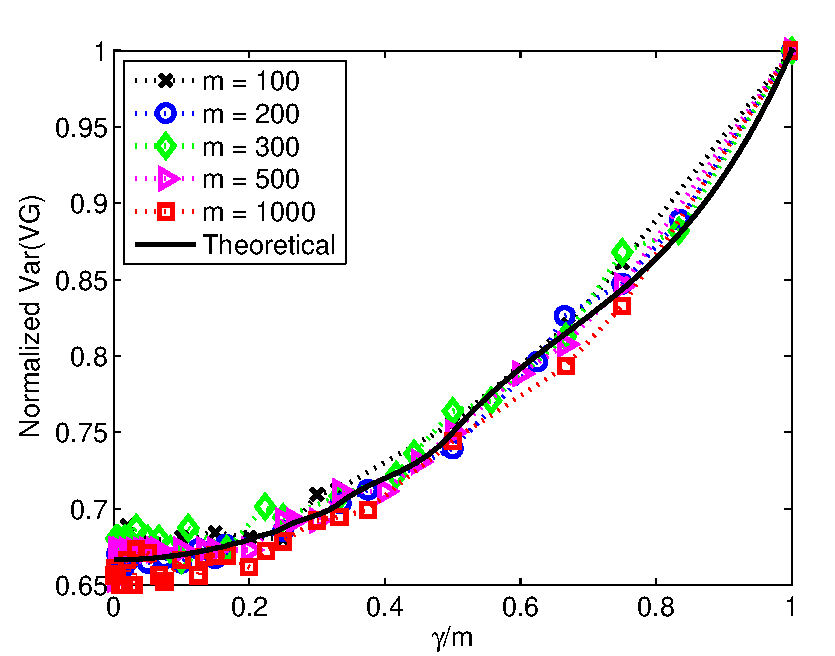
\includegraphics[width=.32\textwidth]{images/nv_varvar_discrete}}
	\subfloat[][Expected Variance]{
	   \label{fig:nv_avgvar}
	   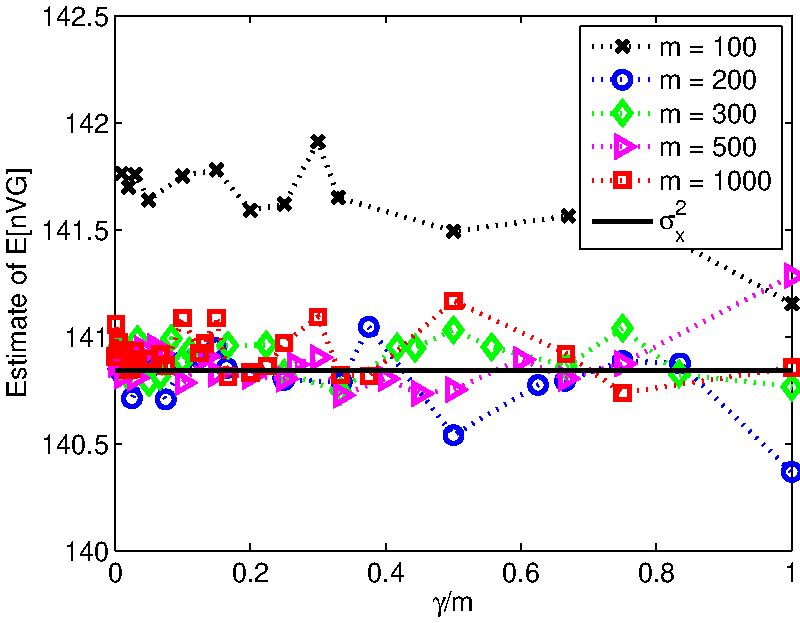
\includegraphics[width=.32\textwidth]{images/nv_avgvar_discrete}}
	\subfloat[][Coverage Probability]{
	   \label{fig:nv_cover}
	   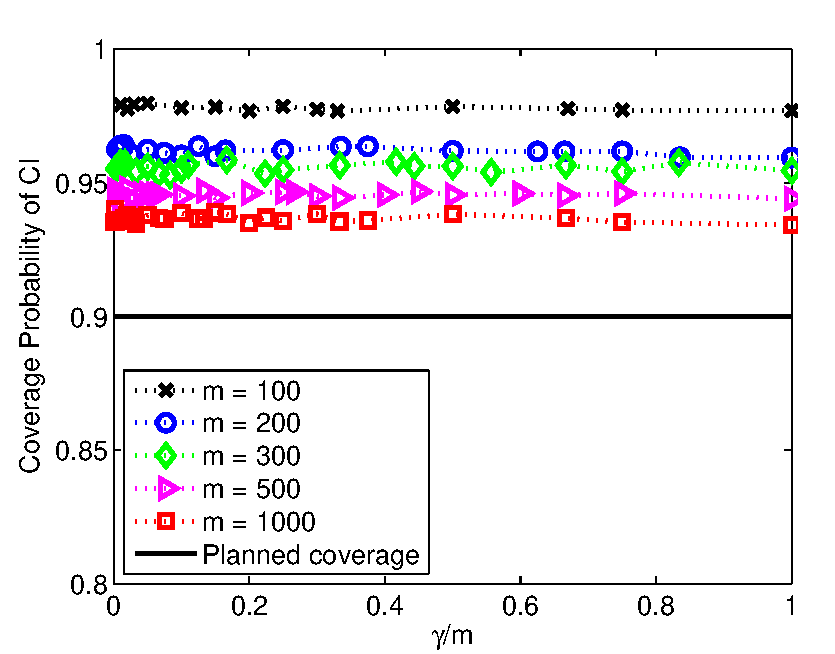
\includegraphics[width=.32\textwidth]{images/nv_cover_discrete}}
	\caption{
		Summary of results for the newsvendor problem. 
		(a) Reduction in variance of $nVG$,
		(b) estimates of $\e{nVG}$, and 
		(c) coverage probability of the confidence intervals for various values of $\gamma/m$ ($\gamma/m=1$ denotes the nonoverlapping batches).
	}
\label{fig:nv}
\end{figure}

\begin{figure}[htb!]
	\centering
	\subfloat[][CEP1]{
	   \label{fig:cep1_varvar}
	   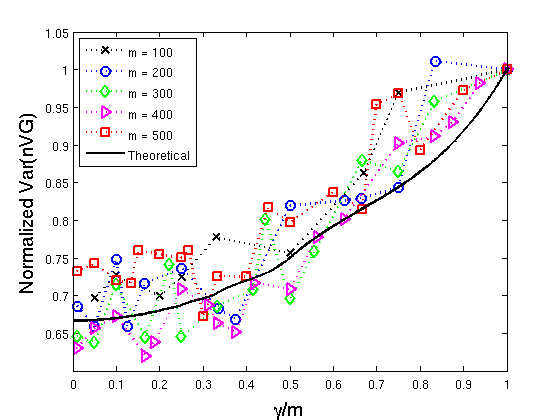
\includegraphics[width=.32\textwidth]{images/cep1_varvar}}
	\subfloat[][10D]{
	   \label{fig:10d_varvar}
	   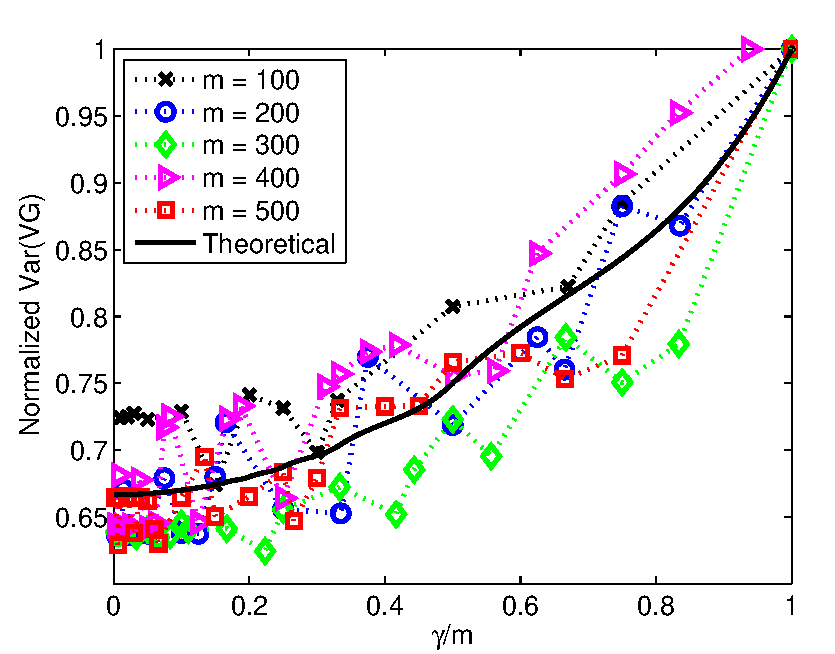
\includegraphics[width=.32\textwidth]{images/10D_varvar}}
		\caption{
		Variance Reduction for
		(a) CEP1 and 
		(b) 10D
		for various values of $\gamma / m$.
		}
\label{fig:varvar}
\end{figure}


Figures~\ref{fig:nv}(a) and \ref{fig:varvar} show the reduction of variance, with each term being normalized with respect to $\var{nVG}$ of the nonoverlapping case (MRP). 
The solid lines in these figures show the theoretical variance reduction from \cite{Welch1987} given by (\ref{eq:var_reduct_formula}). 
Empirical results agree with the theoretical values well, with more variability observed in CEP1 and 10D, providing evidence that similar variance reduction can be achieved in stochastic programming by overlapping the batches even with small sample sizes. 

Figure~\ref{fig:nv}(b) shows estimates of $\e{nVG}$ in the newsvendor problem for changing batch size and amount of overlap. 
We can see that the expectation of the variance estimator is not changed with increasing overlap. 
Although the estimate of $\e{nVG}$ looks large for $m=100$, the error from $\sigma^2_\xh$ is never more than 1\%.  
Estimates for $\e{nVG}$ showed a similar pattern for CEP1 and 10D.  Those graphs are omitted for brevity.

Finally, Figure~\ref{fig:nv}(c) shows the coverage probability of confidence intervals generated by OMRP for several values of $m$ across varying values of $\gamma/m$ for the newsvendor problem.  
The results of the classical overlapping batches estimators show that coverage probability does not change with the amount of overlap, which we can  empirically see in this figure for OMRP for newsvendor, and we observed the same for CEP1 and 10D.  
The coverage probabilities from applying the (nonoverlapping) MRP algorithm to these problems presented in \cite{Bayraksan2006} agree with the our results: for the newsvendor problem, coverage probability drops as $m$ increases and the coverage probability of CEP1 (not shown) remains fairly constant around the desired value of $90\%$. 
Coverage probability for 10D (not shown) was very high, more than $0.99$.  The bias from solving (\ref{eq:sto_prog_m}) for 10D seems to be much more significant than the variance.

Because variance reduction drops quickly as $\gammab$ drops below $1$, the authors recommend using an intermediate value of $\gammab$, such as $1/3$ or $1/4$, to gain the majority of the variance reduction, while reducing the number of optimization problems to be solved. 
Warm-starting the algorithm to solve the sampling problems, when such as scheme is available, can significantly reduce the solution times.


\section{Conclusion} \label{sec:concl}
We have extended previous work from simulation analysis to assessing solution quality in stochastic programming by means of variably overlapping batches \cite{Meketon1984,Song1992,Welch1987} for Monte Carlo sampling-based estimators of optimality gaps in stochastic programs \cite{Mak1999}. 
We have provided conditions under which the resulting point estimator of the optimality gap and its associated sample variance are consistent, the same variance reduction can be achieved, and asymptotically valid confidence intervals can be formed. 
Empirical results with small sample sizes indicate that the asymptotic reductions in variance of the variance estimator show a similar decrease in OMRP, while bias and coverage probability remain unaffected. 


\section*{Acknowledgments}
The authors thank Andrzej Ruszczy{\'{n}}ski and Artur {\'{S}}wietanowski for
access to their regularized decomposition code. 
This research is supported
in part by the National Science Foundation under Grants DMS-0602173 and
EFRI-0835930.  
An earlier version of this paper appeared in \cite{love2011overlapping}.

% Please don't exchange the bibliographystyle style 
\bibliographystyle{plain}
% AUTHOR: Include your bib file here
\bibliography{omrp}

% \section*{AUTHOR BIOGRAPHIES}
 
% \noindent {\bf DAVID LOVE} is a graduate student in the Inderdisciplinary Program in Applied Mathematics at the University of Arizona.  His research focuses on Monte Carlo based quality assessment in stochastic programming.  His email address is \href{mailto://dlove@email.arizona.edu}{dlove@email.arizona.edu}.\\

% \noindent {\bf G\"{U}Z\.{I}N BAYRAKSAN} is an Assistant Professor in the Department of Systems and Industrial Engineering at the University of Arizona. Her research interests include stochastic optimization, particularly Monte Carlo sampling-based methods for stochastic programming, with applications to water resources management. Her email address is \href{mailto://guzinb@sie.arizona.edu}{guzinb@sie.arizona.edu} and her web page is \href{http://www.sie.arizona.edu/faculty/guzinb}{www.sie.arizona.edu/faculty/guzinb}.\\

\end{document}
